\subsection{Experimentos}

Para verificar el $fairness$ de nuestro scheduler decidimos cargarle una determinada cantidad de tareas y comparar cuántos ticks insumía cada una en un rango determinado. Si efectivamente existe ecuanimidad, cada una de las tareas debería insumir una cantidad similar de ticks.

Para testear este comportamiento tomamos el siguiente lote de tareas: una bloqueante y tres que consumen cpu. Las tres insumen en total una cantidad fija de cilos. La bloqueante bloquea 16 veces y las demás tienen un quantum de 32. Como se trata de un scheduler $pseudoaleatorio$ fue necesario realizar el expermimento varias veces con el objetivo de evitar resultados indeseados.

Decidimos tomar como rango inicial el instante en el que todas las tareas ya fueron ejecutadas ya que a partir de allí comenzarán a influir los $compensations \ tickets$. El rango final se determinó de forma arbitraria cersiorándose de que se encuentre antes de la finalización de alguna tarea.

Realizamos el experimento para un scheduler de 1 core y un quantum de 4 y los resultados fueron los siguientes:

\begin{figure}[!h]
	\begin{center}
		  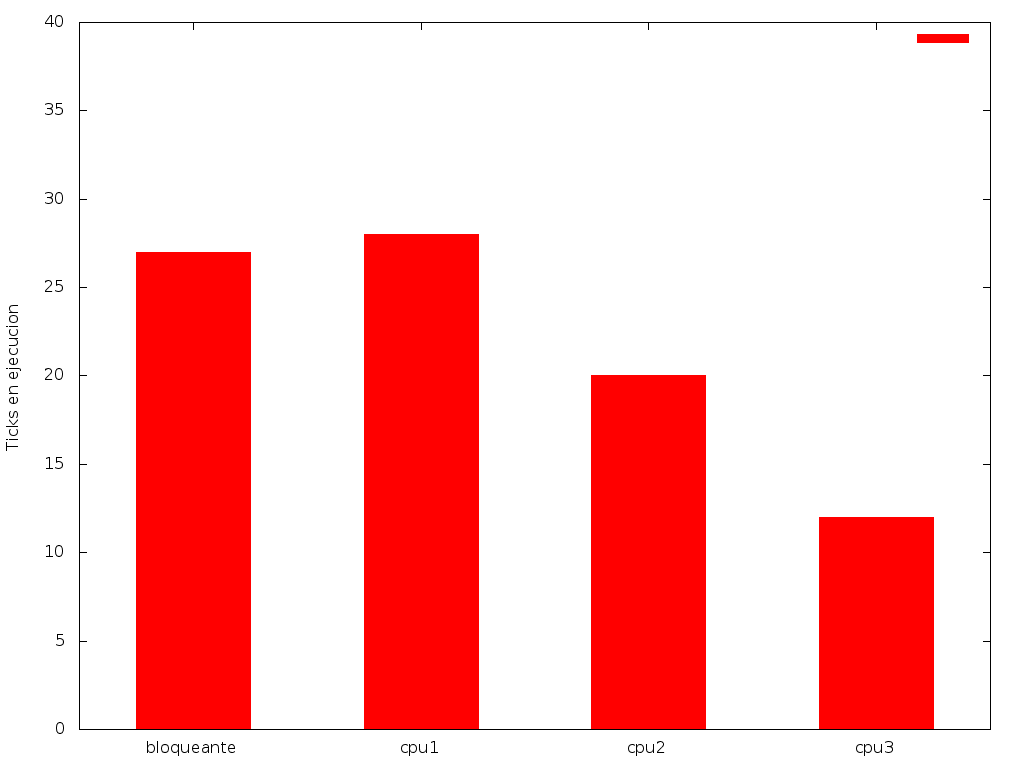
\includegraphics[scale=0.3]{Graficos/comp1.png}
		  \caption{Ticks insumidos por cada tarea para un schedLottery de 4 tareas: 1 bloqueante y 3 de CPU (1 core)}
		  \label{fig:contra1}
	\end{center}
\end{figure}
\FloatBarrier

Para 2 cores ocurrió lo siguiente:

\begin{figure}[!h]
	\begin{center}
		  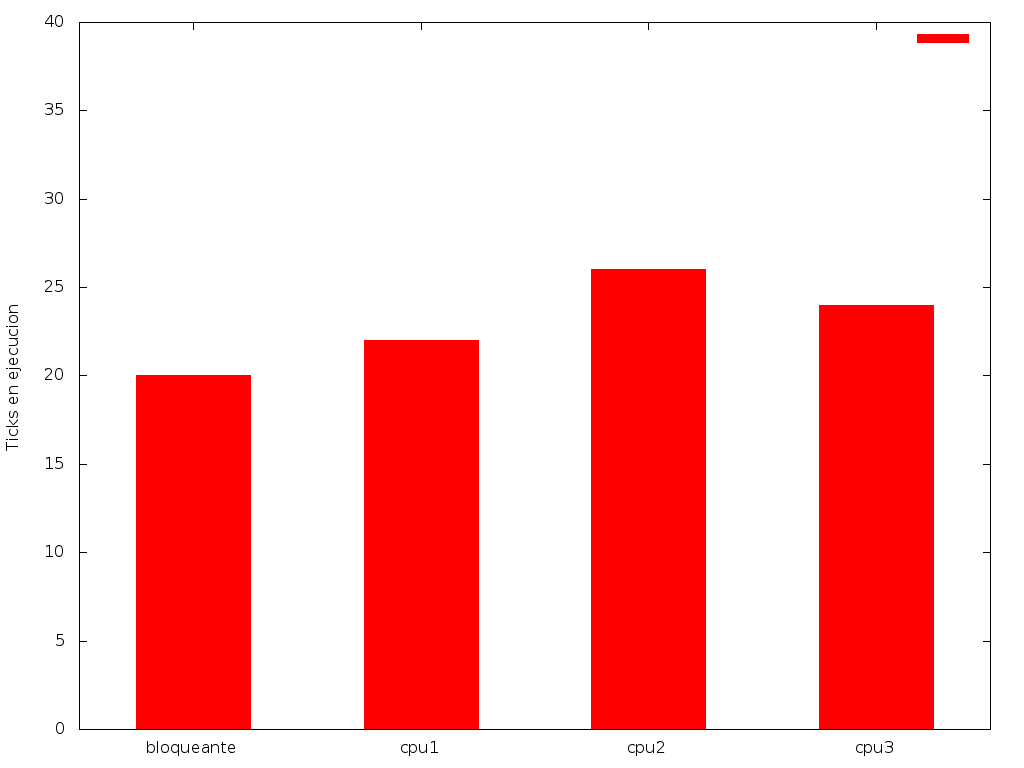
\includegraphics[scale=0.3]{Graficos/comp2.png}
		  \caption{Ticks insumidos por cada tarea para un schedLottery de 4 tareas: 1 bloqueante y 3 de CPU (2 core) }
		  \label{fig:contra1}
	\end{center}
\end{figure}
\FloatBarrier

Como se puede observar, los ticks insumidos por cada tarea es bastante equitativa. Esto quiere decir que los $compensation \ tickets$ están actuando a favor de la tarea bloqueante que es la que utiliza solo una parte de su quantum cada vez que se ejecuta.

Los $compensation \ tickets$ son los que lo otorgan equanimidad a este scheduler. Sin ellos la tarea bloqueante no hubiera insumido los ticks que insumió en las pruebas anteriores. Para comprobar esto, corrimos el mismo scheduler con el mismo lote de tareas pero sin $compensation \ tickets$. Estos fueron los resultados:

Para 1 core:

\begin{figure}[!h]
	\begin{center}
		  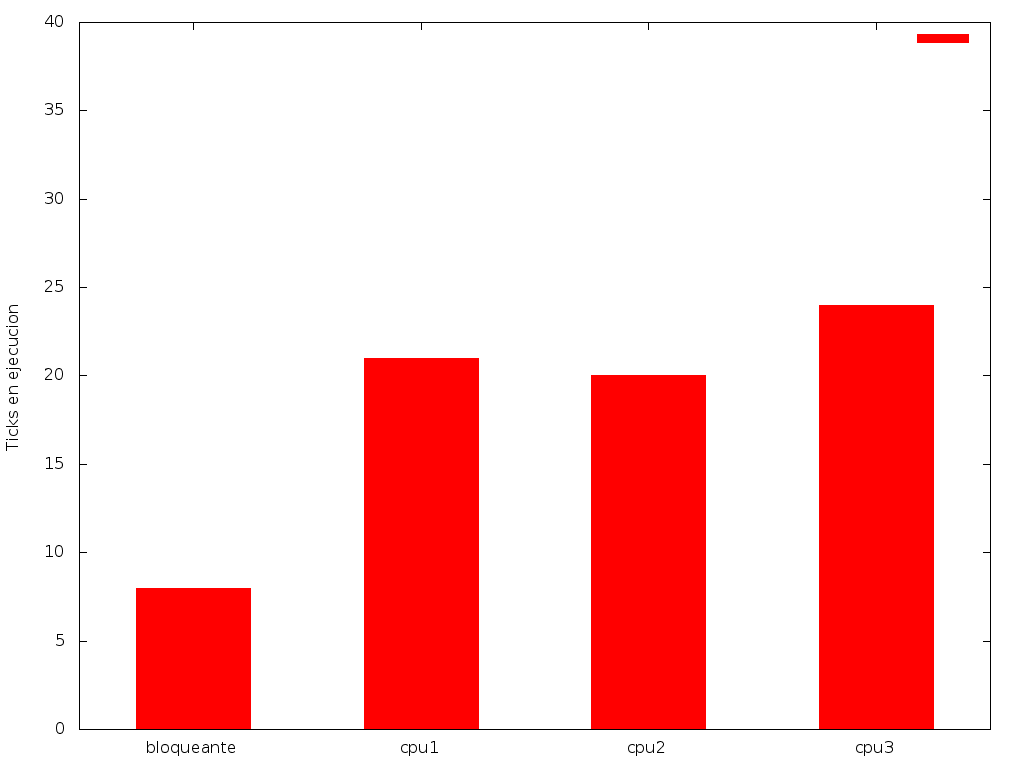
\includegraphics[scale=0.3]{Graficos/sincomp1.png}
		  \caption{Ticks insumidos por cada tarea para un schedLottery de 4 tareas: 1 bloqueante y 3 de CPU (1 core). Sin $compensation \ tickets$}
		  \label{fig:contra1}
	\end{center}
\end{figure}
\FloatBarrier

Para 2 cores:

\begin{figure}[!h]
	\begin{center}
		  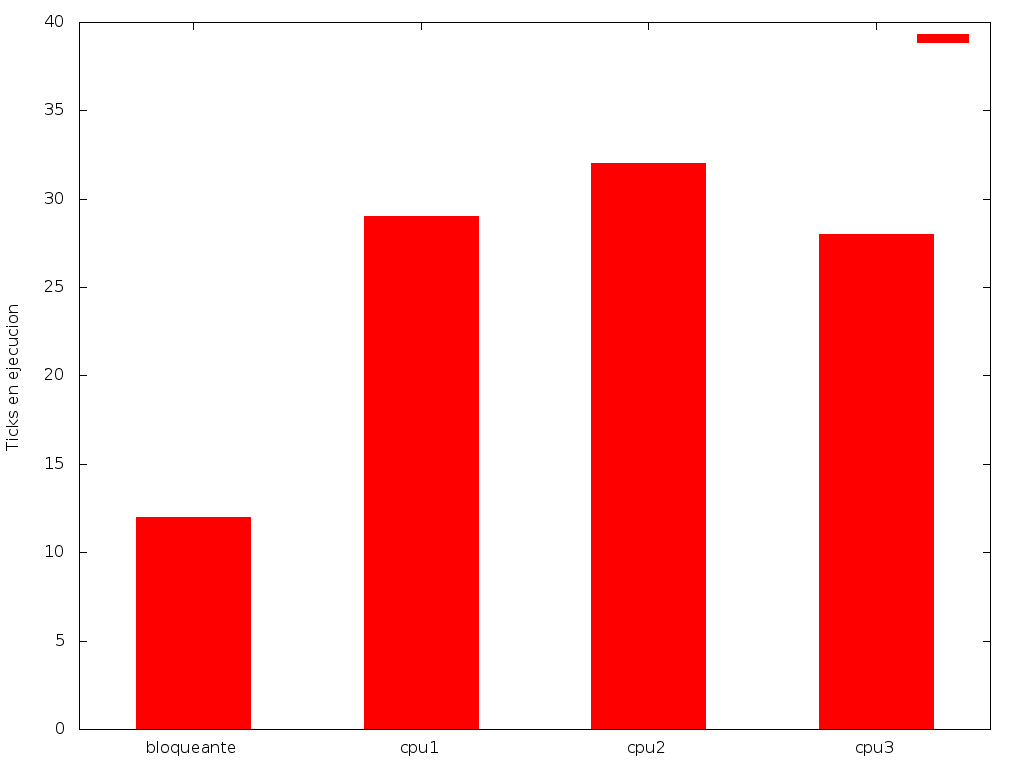
\includegraphics[scale=0.3]{Graficos/sinComp2.png}
		  \caption{Ticks insumidos por cada tarea para un schedLottery de 4 tareas: 1 bloqueante y 3 de CPU (1 core). Sin $compensation \ tickets$}
		  \label{fig:contra1}
	\end{center}
\end{figure}
\FloatBarrier

Como puede oservarse, los ticks insumidos por la tarea bloqueante es mucho menor de lo que era antes. La ecuanimidad ya no está presente en este scheduler.
